% Template for ICASSP-2020 paper; to be used with:
%          spconf.sty  - ICASSP/ICIP LaTeX style file, and
%          IEEEbib.bst - IEEE bibliography style file.
% --------------------------------------------------------------------------
%\usepackage{multicol}
%\usepackage{multirow}
\documentclass{article}
\usepackage{color}
\usepackage{booktabs}
\usepackage{amsfonts}
\usepackage{spconf,amsmath,graphicx}
\usepackage{tikz}
\usepackage{pgfplots}
\usepackage{subfig}
\usepackage{float}
%\usepackage[preprint]{spconf}
\usepackage[OT1]{fontenc} % TODO: 之後放到 overleaf 要移掉!!

% Example definitions.
% --------------------
\def\x{{\mathbf x}}
\def\L{{\cal L}}
\pgfplotsset{compat=1.16}

% ------
\title{Meta Learning for End-to-End Low-Resource Speech Recognition}
%
% Single address.
% ---------------
%\name{Jui-Yang Hsu, Yuan-Jui Chen,  Hung-yi Lee}
\name{Jui-Yang Hsu\qquad Yuan-Jui Chen\qquad  Hung-yi Lee}
\address{National Taiwan University \\
\small{\texttt{\{r07921053, r079xxxxx, hungyilee\}@ntu.edu.tw}}}
%
% For example:
% ------------
%\address{School\\
%	Department\\
%	Address}
%
% Two addresses (uncomment and modify for two-address case).
% ----------------------------------------------------------
%\twoauthors
%  {A. Author-one, B. Author-two\sthanks{Thanks to XYZ agency for funding.}}
%	{School A-B\\
%	Department A-B\\
%	Address A-B}
%  {C. Author-three, D. Author-four\sthanks{The fourth author performed the work
%	while at ...}}
%	{School C-D\\
%	Department C-D\\
%	Address C-D}
%
\begin{document}
%\ninept
%
\maketitle
%
\begin{abstract}
  \textcolor{red}{(TBD BEGIN)} With the recent advances of deep learning, integrating the main modules of automatic speech recognition (ASR) such as acoustic model, pronunciation lexicon and language model into a single end-to-end model is highly attractive. Connectionist Temporal Classification (CTC) lends itself on such end-to-end approach by introducing an additional blank symbol and specifically-designed loss function optimizing to generate the correct character sequences from the speech signal directly, without framewise phoneme alignment in advance. With many recent results, end-to-end deep learning has created larger interest in speech community. \textcolor{red}{(TBD END)}
\end{abstract}
%
\begin{keywords}
  meta-learning, low-resource, multi-lingual speech recognition, language adaptation, IARPA-BABEL
\end{keywords}
%
\section{Introduction}
\label{sec:intro}

With the recent advances of deep learning, integrating the main modules of automatic speech recognition (ASR) such as acoustic model, pronunciation lexicon, and language model into a single end-to-end model is highly attractive. Connectionist Temporal Classification (CTC) \cite{graves2006connectionist} lends itself on such end-to-end approaches by introducing an additional blank symbol and specifically-designed loss function optimizing to generate the correct character sequences from the speech signal directly, without framewise phoneme alignment in advance. With many recent results \cite{hannun2014deep, amodei2016deep, collobert2016wav2letter}, end-to-end deep learning has created a larger interest in the speech community.

However, the end-to-end ASR system requires a huge amount of paired speech-transcription data, which is costly. 
For most languages in the world, they lack sufficient paired data for training. 
Pretraining on other language sources as the initialization, then fine-tuning on target language is the dominant approach in such low-resource settings, also known as multilingual transfer learning / pretraining (MultiASR) \cite{vu2014multilingual, tong2017investigation}. 
The backbone of MultiASR is a multitask model with shared hidden layers (encoder), and many language-specific heads. 
The model structure is designed to learn an encoder to extract language-independent representations to build a better acoustic model from many source languages. 
The success of ``language-independent'' features to improve ASR performance compared to monolingual training has been shown in many recent works \cite{cho2018multilingual, dalmia2018sequence}.

\begin{figure}[htb]

\begin{minipage}[b]{0.48\linewidth}
  \centering
  \centerline{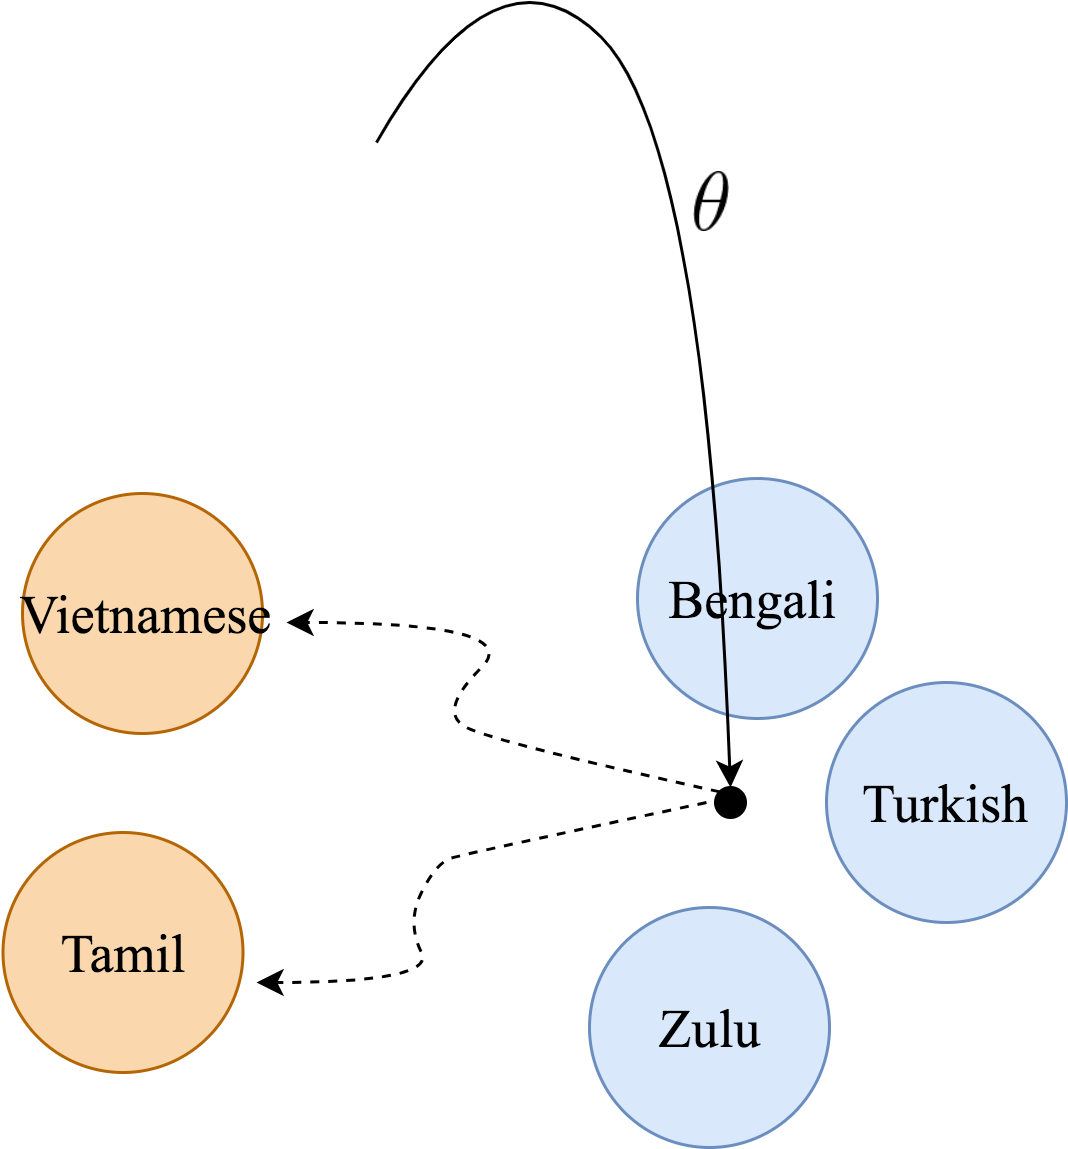
\includegraphics[width=4.0cm]{figs/multi_process.png}}
%  \vspace{1.5cm}
  \centerline{(a) MultiASR}\medskip
\end{minipage}
\hfill
\begin{minipage}[b]{0.48\linewidth}
  \centering
  \centerline{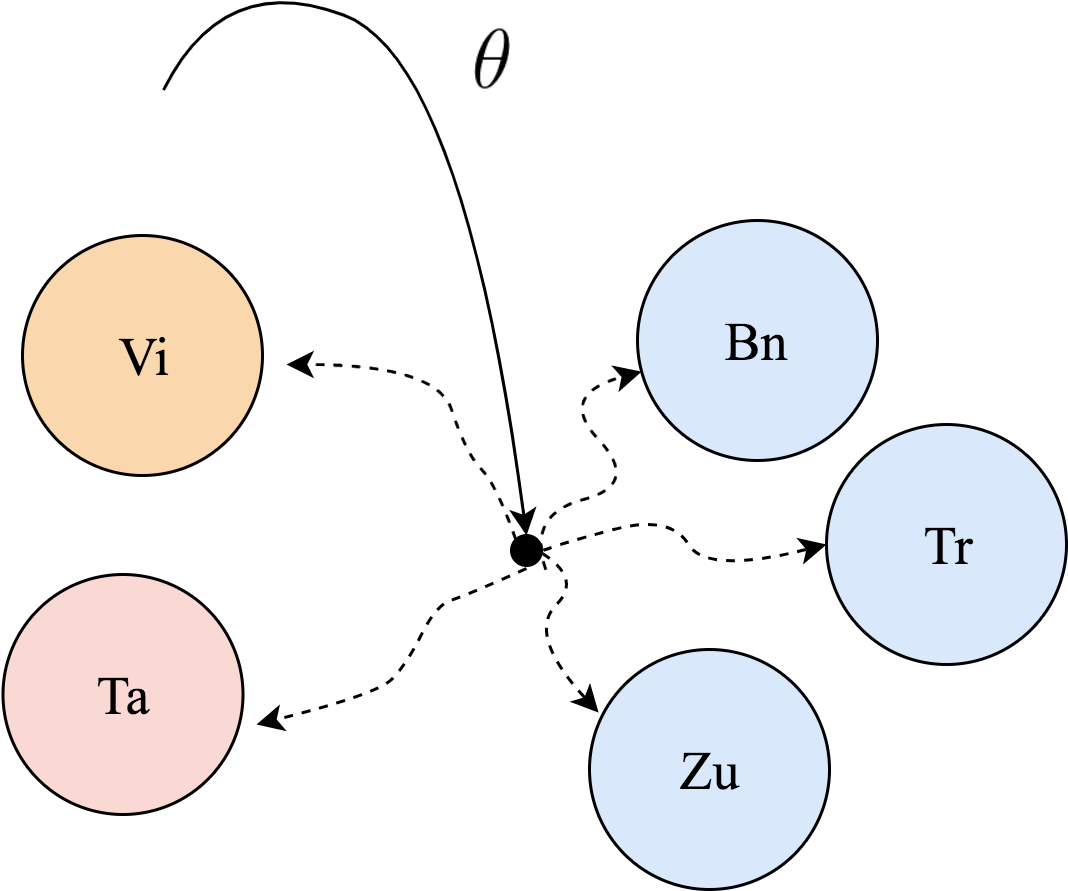
\includegraphics[width=4.0cm]{figs/meta_process.png}}
%  \vspace{1.5cm}
  \centerline{(b) MetaASR}\medskip
\end{minipage}
%
\caption{Illustration: Difference of the learned parameters from MultiASR \& MetaASR. The solid lines represent the learning process of pretraining, either multitask or meta learning. The dashed lines represent the language-specific adaptation.\\ (The figure is modified from \cite{gu2018meta})}
\label{fig:meta-idea}
%
\end{figure}



Besides directly training the model with all the source languages, there are various variants of MultiASR approaches. 
Language-adversarial training approaches \cite{Yi2018AdversarialMT, adams2019massively} introduce language-adversarial classification objective to the shared encoder, negating the gradients backpropagated from the language classifier to encourage the encoder to extract more language-independent representations. 
Hierarchical approaches \cite{Sanabria2018HierarchicalMT} introduce different granularity objectives by combining both character and phoneme prediction at different levels of the model.

%Lee: 我暫時把兩段合併,這邊應該要提到說,我們用的方法是 MAML ,可以跟任何 network architecture 結合
In this paper, we provide a novel research direction following up on the idea of multilingual pretraining -- \textbf{Meta learning}. 
Meta learning, or learning-to-learn, has recently received considerable interest in the machine learning community. The goal of meta learning is to solve the problem of ``fast adaptation on unseen data'', which is aligned with our low-resource setting.
 With its success in computer vision under the few-shot learning setting~\cite{rusu2018meta, snell2017prototypical, vinyals2016matching}, there have been some works in language and speech processing, for instance, language transfer in neural machine translation \cite{gu2018meta}, dialogue generation \cite{mi2019meta}, and speaker adaptive training \cite{klejch2018learning}, but not multilingual pretraining for speech recognition.

We use model-agnostic meta-learning algorithm (MAML) \cite{finn2017model} in this work. 
As its name suggested, MAML can be applied to any network architecture. 
MAML only modifies the optimization process following meta learning training scheme.
It does not introduce additional modules like adversarial training or requires phoneme level annotation (usually through lexicon) like hierarchical approaches. 
We evaluated the effectiveness of the proposed meta learning algorithm, MetaASR, on the IARPA BABEL dataset \cite{gales2014speech}. Our experiments reveal that MetaASR outperforms MultiASR significantly across all target languages.
\section{Proposed Approach}
\label{sec:approach}

Meta meta \cite{finn2017model}


\section{Experiment}
\label{sec:exp}

%\subsection{Experimental Setup}
\label{ssec:exp-setup}
In this work, we used data from the IARPA BABEL project \cite{gales2014speech}. The corpus is mainly composed of conversational telephone speech (CTS). We selected 6 languages as non-target languages for multilingual pre-training: Bengali (Bn), Tagalog (Tl), Zulu (Zu), Turkish (Tr), Lithuanian (Lt), Guarani (Gn), and 4 target languages for adaptation: Vietnamese (Vi), Swahili (Sw), Tamil (Ta), Kurmanji (Ku), and experimented different combinations of non-target languages for pretraining.

We followed the recipe provided by Espnet \cite{watanabe2018espnet} for data preprocessing and final score evaluation.  We used 80-dimensional Mel-filterbank and 3-dimensional pitch features as acoustic features. The size of the sliding window is 25ms, and the stride is 10ms. We used the shared encoder with 6-layer VGG extractor with downsampling and a 6-layer bidirectional LSTM network with 360 cells in each direction used in the previous work \cite{dalmia2018sequence}.

%\subsubsection{Pretraining} # TODO: move to approach
%\vspace{-5pt}
\begin{table*}[ht!]
\centering
\caption{Character error rate (\si{\percent} CER) w.r.t the pretraining languages set for all 4 target languages' LLP}
\label{tab:llp-table}
\begin{tabular}{@{}ccccccccc@{}}
%\begin{tabular}{l|cc|cc|cc|cc}
\toprule
Model                                    & \multicolumn{2}{c}{Vietnamese}                         & \multicolumn{2}{c}{Swahili}                        & \multicolumn{2}{c}{Tamil}                        & \multicolumn{2}{c}{Kurmanji} \\

                                         & multi           & meta                                & multi           & meta                                & multi           & meta                                & multi           & meta           \\ \midrule
\multicolumn{1}{c|}{(no-pretrain)}                   & \multicolumn{2}{c|}{-}                    & \multicolumn{2}{c|}{-}                    & \multicolumn{2}{c|}{-}          & \multicolumn{2}{c}{-}                    \\

\multicolumn{1}{l|}{Bn Tl Zu}   & -          & \multicolumn{1}{c|}{-}          & -          & \multicolumn{1}{c|}{-}          & -          & \multicolumn{1}{c|}{-}          & -          & -          \\
\multicolumn{1}{l|}{ \qquad \qquad Tr Lt Gn} & -          & \multicolumn{1}{c|}{-}          & -          & \multicolumn{1}{c|}{-}          & -          & \multicolumn{1}{c|}{-}          & -          & -          \\
\multicolumn{1}{l|}{Bn Tl Zu Tr Lt Gn}           & -          & \multicolumn{1}{c|}{-}          & -          & \multicolumn{1}{c|}{-}          & -          & \multicolumn{1}{c|}{-}          & -          & -          \\ \bottomrule
%\multicolumn{1}{c|}{MLing + SWBD \& FT}       & \textbf{48.2} & \multicolumn{1}{c|}{\textbf{33.5}} & \textbf{48.7} & \multicolumn{1}{c|}{\textbf{31.9}} & \textbf{44.3} & \multicolumn{1}{c|}{\textbf{31.9}} & \textbf{51.5} & \textbf{37.8} \\ \bottomrule
\end{tabular}
\end{table*}


\begin{table*}[ht!]
\centering
\caption{Character (\% CER)  error rate w.r.t the pretraining languages set for all 4 target languages' FLP}
\label{tab:block-results}
\begin{tabular}{@{}ccccccccc@{}}
%\begin{tabular}{l|cc|cc|cc|cc}
\toprule
Model                                    & \multicolumn{2}{c}{Vietnamese}                         & \multicolumn{2}{c}{Swahili}                        & \multicolumn{2}{c}{Tamil}                        & \multicolumn{2}{c}{Kurmanji} \\

                                         & multi           & meta                                & multi           & meta                                & multi           & meta                                & multi           & meta           \\ \midrule
\multicolumn{1}{c|}{- (no-pretrain)}         & 100.0          & \multicolumn{1}{c|}{100.0}          & 100.0          & \multicolumn{1}{c|}{100.0}          & 100.0          & \multicolumn{1}{c|}{100.0}          & 100.0          & 100.0          \\

\multicolumn{1}{c|}{Bn Tl Zu}   & 53.2          & \multicolumn{1}{c|}{36.5}          & 52.8          & \multicolumn{1}{c|}{34.4}          & 47.8          & \multicolumn{1}{c|}{34.9}          & 55.9          & 41.1          \\
\multicolumn{1}{c|}{ Tr Lt Gn} & 50.6          & \multicolumn{1}{c|}{35.1}          & 49.0          & \multicolumn{1}{c|}{32.2}          & 46.6          & \multicolumn{1}{c|}{33.2}          & 53.4          & 39.6          \\
\multicolumn{1}{c|}{Bn Tl Zu Tr Lt Gn}           & 52.3          & \multicolumn{1}{c|}{36.6}          & 51.3          & \multicolumn{1}{c|}{33.0}          & 45.8          & \multicolumn{1}{c|}{33.9}          & 54.5          & 40.2          \\ \bottomrule
%\multicolumn{1}{c|}{MLing + SWBD \& FT}       & \textbf{48.2} & \multicolumn{1}{c|}{\textbf{33.5}} & \textbf{48.7} & \multicolumn{1}{c|}{\textbf{31.9}} & \textbf{44.3} & \multicolumn{1}{c|}{\textbf{31.9}} & \textbf{51.5} & \textbf{37.8} \\ \bottomrule
\end{tabular}
\end{table*}



% (TODO) Hsu:Need to discussed use one or use three?
% (TODO) Hsu: 最後一句超遨口的...叫 dev set 會不會太隨便?
\subsection{Validation Languages}
We used Limited Language Pack (LLP) which consists of 10\% Full Language Pack (FLP) of the other 3 languages to determine which pretraining step we should pick as the pretrained model for adapting on certain language's LLP and FLP. (For instance, when adapting on Vi, we use Sw, Ta, Ku s' LLP validation set as the validation set for Vi)

\subsection{Meta Learning}
For each meta learning episode, we use a single gradient step of language-specific learning with SGD when computing the meta gradient. Noted that in Eq. \ref{eq:meta-grad}, if we expand the loss term in the summation, we will find the second derivative term of $\theta$ appear. For computation efficiency, some previous works \cite{finn2017model, nichol2018reptile} showed that we could ignore the second-order term without affecting the performance too much. Therefore, we approximate Eq. \ref{eq:meta-grad} as follows.

\begin{equation}
  \theta \leftarrow \theta - \eta^\prime \sum_k \nabla_{\textcolor{red}{\theta^\prime}} \mathcal{L}_{D^\prime_k}(\theta^\prime)
\end{equation}
Also known as First-order MAML (FOMAML).

\subsection{Fine-Tuning (Adaptation) and Evaluation}
For adaptation on target language, we fine-tuned each monolingual model for 20 epochs for LLP, 18 epochs for FLP, and early-stopped on its own dev set, and evaluated on its test set. 
%We report the results in Table \ref{tab:llp-table} and \ref{tab:flp-table}.


\section{Results}
\label{sec:results}

\subsection{vs. Multitask Learning (MultiASR)}
\label{ssec:baseline-multitask}

\subsection{Training Set Size}
\label{ssec:training-size}








\section{Conclusion}
\label{sec:conclusion}

\textcolor{red}{TBD BEGIN}All is well \textcolor{red}{TBD END}



% Below is an example of how to insert images. Delete the ``\vspace'' line,
% uncomment the preceding line ``\centerline...'' and replace ``imageX.ps''
% with a suitable PostScript file name.
% -------------------------------------------------------------------------


% To start a new column (but not a new page) and help balance the last-page
% column length use \vfill\pagebreak.
% -------------------------------------------------------------------------
%\vfill
%\pagebreak


%\section{REFERENCES}
% References should be produced using the bibtex program from suitable
% BiBTeX files (here: strings, refs, manuals). The IEEEbib.bst bibliography
% style file from IEEE produces unsorted bibliography list.
% -------------------------------------------------------------------------
\bibliographystyle{IEEEbib}
\newpage
\bibliography{strings,refs}

\end{document}
